\chapter{Introduzione alla sicurezza di rete}

\dfn{Sicurezza di rete}{
    La sicurezza di rete è l'insieme delle strategie, tecnologie e protocolli utilizzati per proteggere le reti di calcolatori da accessi non autorizzati, attacchi, perdite di dati e altre minacce informatiche
}

In pratica consiste nel creare un'architettura di difesa e prevenzione. Questi sono in modo riassuntivo i principali obbiettivi della sicurezza di rete:
\begin{itemize}
    \item \textbf{Confidenzialità}: Solo il mittente e il destinatario devono poter leggere il messaggio. Questo si ottiene con la crittografia
    \begin{itemize}
        \item Il mittente crittografa (encrypts) il messaggio.
        \item Il destinatario decrittografa (decrypts) il messaggio
    \end{itemize}
    \item \textbf{Autenticazione}: Processo per verificare l’identità di un utente o un dispositivo, fondamentale per garantire accessi sicuri (es. Password, certificati digitali, autenticazione a due fattori (2FA))
    \item \textbf{Integrità dei messaggi}: Garantisce che i dati non siano stati alterati durante la trasmissione (es. Password, certificati digitali, autenticazione a due fattori (2FA))
    \item \textbf{Accesso e Disponibilità}: I servizi devono essere accessibili agli utenti autorizzati. Minacce:
    \begin{itemize}
        \item Attacchi DoS/DDoS che bloccano il servizio.
        \item Gestione dei permessi per prevenire accessi non autorizzati
    \end{itemize}
\end{itemize}

Si introduce il concetto di attacco con il tipico esempio di Alice e Bob che vogliono comunicare e Trudy, l'attaccante, che può intercettare, elliminare o aggiungere messaggi durante la comunicazione dei due amamnti carucci (Morbidelli - Morigi)
\begin{center}
    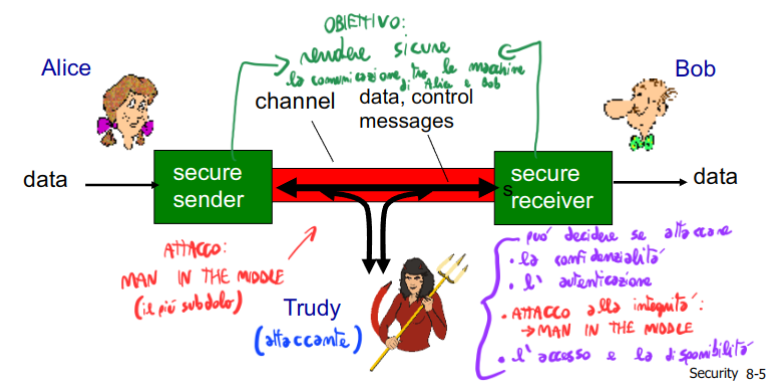
\includegraphics[width=10cm]{img/trudy_bob_alice.png}
\end{center}

Vabbuò passiamo alla sezione sucessiva:
\section{Principi di crittografa}
Partiamo dalla defnizione

\dfn{crittografa}{
    si \textbf{crittografa} la disciplina che studia le tecniche per proteggere le informazioni trasformandole in un formato illeggibile per chi non è autorizzato, consentendo solo ai destinatari legittimi di decifrarle.
}

Nelle reti di comunicazione, i dati trasmessi possono essere intercettati da chiunque abbia accesso al canale di comunicazione, rendendo le informazioni vulnerabili a lettura, modifica o attacchi malevoli. Per proteggere la riservatezza e l’integrità dei dati, si utilizza, quindi, la crittografia, una tecnica che consente di trasformare il testo in chiaro, detto \textit{plaintext}, in un formato incomprensibile chiamato testo cifrato o \textit{ciphertext}, attraverso l’applicazione di un algoritmo di cifratura.

L’obiettivo della crittografia è garantire che, anche se un malintenzionato intercettasse il messaggio durante la trasmissione, non sarebbe in grado di comprenderne il contenuto senza la conoscenza della chiave segreta. Solo il destinatario legittimo, in possesso della chiave corretta, può applicare un algoritmo di decifratura per convertire il testo cifrato nuovamente in testo leggibile.

Va sottolineato che gli algoritmi di cifratura e decifratura sono generalmente pubblici e noti a tutti. Tuttavia, la sicurezza della crittografia si basa sulla segretezza della cosiddetta \textit{chiave crittografica}, ovvero una sequenza di bit utilizzata all'interno di un algoritmo di cifratura per trasformare un messaggio in un formato sicuro e, successivamente, per riconvertirlo nel suo stato originale. Questa chiave viene generata all'inizio della comunicazione tra mittente e destinatario e loro e solo loro ne sono a conoscenza.

Adesso un'introduzione all'algebra della crittografia

Si ha:
\begin{itemize}
    \item $m$: plaintext
    \item $K_A(m)$: ciphertext, encrypted with key $K_A$
    \item $m = K_B(K_A(m))$: plaintext ripristinato grazie alla chiave $K_B$
\end{itemize}

Si noti la seguente immagine (con appunti bonziani):
\begin{center}
    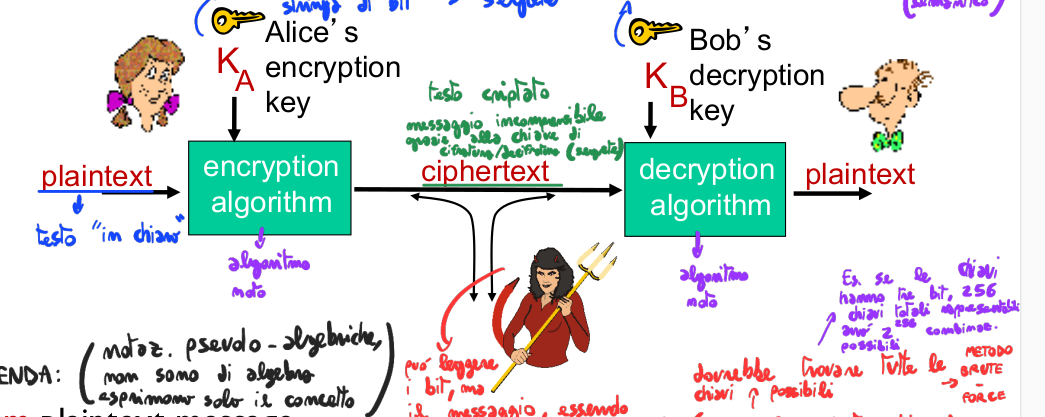
\includegraphics[width=10cm]{img/crittografia.png}
\end{center}

\subsection{Attaccare uno schema di crittografia}

Gli attacchi crittografici mirano a violare la sicurezza di un sistema di cifratura. Ne esistono diversi tipi:
\begin{enumerate}
    \item \textbf{Cipher-text only attack}, l'attaccante possiede solo il testo cifrato a disposizione e per decifrare il messaggio ha due approcci possibile:
    \begin{itemize}
        \item \textbf{Forza bruta}: prova tutte le chiavi possibili
        \item \textbf{Analisi statistica}: cerca pattern ripetuti nei dati cifrati
    \end{itemize}
    \item \textbf{known-plaintext attack}: Trudy possiede sia il testo cifrato che il corrispondente testo in chiaro. Con queste informazioni, cerca di scoprire la chiave di cifratura o il meccanismo utilizzato, così da poter decifrare altri messaggi cifrati dallo stesso sistema.
    
    \ex{}{
    Se Trudy sa che nel testo in chiaro compare la parola "hello" e trova nel messaggio cifrato la sequenza "JGRRG", può iniziare a costruire un dizionario di corrispondenze tra lettere:

    \begin{itemize}
        \item $h \to J$
        \item $e \to G$
        \item $l \to R$
        \item $o \to G$
    \end{itemize}
    }
    
\end{enumerate}

\nt{un buon metodo per evitare questi attacchi è rendere lo spazio delle chiavi il più vasto possibile e utilizzare algoritmi sicuri che resistano alle analisi statistiche}
\subsection{Crittografia a chiave simmetrica}
Adesso entriamo nel vivo della difesa cazzo
\dfn{Crittografia a chiave simmetrica}{
    mittente e destinatario condividono la stessa chiave segreta $K_S$ per cifrare e decifrare i messaggi
}

I pratica il mittente (Alice) cirfra il plaintext con l'algoritmo di cifratura usando la chiave $K_S$ottenendo il ciphertext, Bob riceve il ciphertext e lo decifra usando lo stesso algoritmo e la chiave $K_S$, recuperando il messaggio originale
\begin{center}
    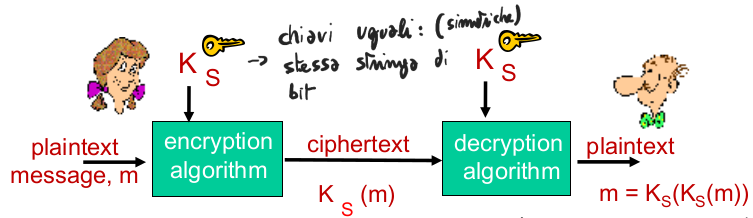
\includegraphics[width=10cm]{img/CHIAVE_SIMMETRICA.png}
\end{center}

Per implementare la chiave simmetrica esistono diverse tecniche

\subsubsection{Cifrario a sostituzione}

\dfn{Cirfrario a sostituizione}{
    Un \textbf{cifrario a sostituzione} è una tecnica di cifratura in cui ogni lettera del testo in chiaro viene sostituita con un'altra lettera secondo un mapping predefinito
}

\paragraph{Cifrario monolitico}
Tra i vari tipi di cifrario a sostruzioni vi è il cifrario monolitico dove ogni lettera dell'alfabeto viene sostituita da un'altra lettera fissa

\ex{Cifrario monolitico}{
    \begin{itemize}
        \item Alfabeto in chiaro: abcdefghijklmnopqrstuvwxyz

        \item Alfabeto cifrato: mnbvcxzasdfghjklpoiuytrewq
        \item Messaggio originale: bob. i love you. alice
        \item Messaggio cifrato: nkn. s gktc wky. mgsbc
    \end{itemize}
}

La chiave di cifratura è una funzione di permutazione ad un insieme di 26 lettere ad un altro insieme di 26 lettere

Tuttavia è poco sicuro perché mantiene la frequenza delle lettere originali e lo rende particolarmente vulnerabile alle analisi delle frequenze

\paragraph{Schema ciclico} Per rendere la cifratura più sicura, si può usare più cifrari di sostituzione e applicarli in un ciclo predefinito

La chiave di cifratura quindi è un insieme di $n$ cifrari sostituzione ($M_1,M_2,\dots,M_n$) ed un modello cicilico su come usarli. Ogni lettera del plaintext quindi viene cifrata con un cifrario diverso seguendo il ciclo 

\section{Firewall e IDS}

Innanzi definiamo che cos'è un \textit{Firewall}

\dfn{Firewall}{
        Si definisce \textbf{Firewall} un sistema di sicurezza che isola una rete interna di un'organizzazione da internet, controllando e filtrando il traffico di rete in entrata e uscita in base a regole di sicurezza definite dette di \texttt{ACCESS} o \texttt{DENIED}
}

L'idea del Firewall è che l'esterno di una rete è composta dai cosiddetti "cattivi ragazzi" che la mamma non vi raccomanderebbe come compagni d'uscita, mentre l'interno della rete è composta da "bravi ragazzi" di cui fidarsi, lo scopo del sistema è, quindi, separare i buoni dai cattivi

\begin{center}
    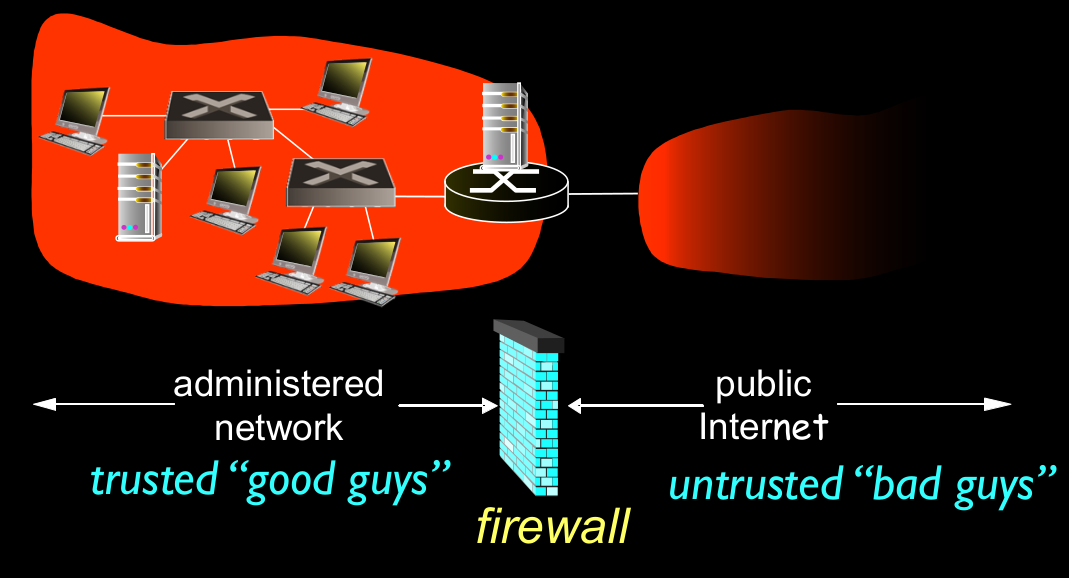
\includegraphics[width=10cm]{img/buoni_cattivi_e_firewall.png}
\end{center}

Il Firewall si rivela utile per principalmente tre motivi:
\begin{itemize}
    \item \textbf{Prevenzione degli attacchi Denial of Service (Dos)}: tipologia di attacco informatico che mira a rendere inaccessibili o indisponibili i servizi di una rete ad utenti legittimi
    
    Un esempio è il \textbf{SYN flooding} in cui un attaccante invia molte richieste di connessione false, esaurendo le risorse del server sovraccaricandolo e impedendo connessioni legittime

    \item \textbf{Protezione dei dati interni da accessi non autorizzati}: ovvero impedisce che gli attaccanti possona \textit{modificare o rubare dati sensibili}
    
    Un esempio classico è un attaccante che sostituisce il sito web di un'organizzazione con un contenuto malevolo.

    \item \textbf{Accesso selettivo e autorizzato alla rete interna}: Permette l’accesso solo a utenti o dispositivi autenticati, migliorando la sicurezza
\end{itemize}

Esistono tre tipi di tipoligie di Firewall che approfonoidremo nel dettaglio:
\begin{itemize}
    \item \textbf{Stateless Packet Filter}: Controlla ogni pacchetto singolarmente, senza tenere traccia delle connessioni
    \item \textbf{Statefull Packet Filter}: Tiene traccia dello stato delle connessioni (es. richieste e risposte)  
    \item \textbf{Application Gateway} (proxy Firewall): controlla il traffico a livello applicativo (es. HTTP, FTP, e.mail), filtrando così le informazioni che all'interno dei protocolli del livello (ad esempio il contenuto di una mail)
\end{itemize}

Si notino nel dettaglio
\subsection{Stateless Packet Filtering}

\dfn{Stateless Packet Filtering}{
    Lo \textbf{Stateless Packet Filtering} è una tecnica di sicurezza di rete in cui un firewall esamina ogni pacchetto individualmente, senza tener conto delle connessioni stabilite in precedenza. Questo significa che ogni pacchetto è valutato isolatamente sulla base di un insieme di regole predefinite
}
Di solito un firewall con filtraggio stateless è implementato su un router che collega una rete interna a internet. Il router analizza ogni pacchetto in ingresso e in uscita e decide se bloccarlo o lasciarlo in base a regole definite nelle cosiddette "\textbf{white list}" (pacchetti che possono passare) e o "\textbf{black list}" (lista di pacchetti da bloccare)

Il firewall prende decisioni basandosi su parametri del pacchetto, tra cui:
\begin{itemize}
    \item \textbf{IP} del mittente e destinatario
    \item \textbf{Numero di porta TCP/UDP} del mittente e destinatario
    \item \textbf{Tipo di messaggio ICMP} bloccando, ad esempio, attacchi di scansione provenienti dall'esterno
    \item \textbf{bit SYN e ACK nei pacchetti TCP}: Il firewall può, ad esempio, bloccare pacchetti con SYN in entrata per impedire connessioni indesiderate dall'esterno
\end{itemize}

Qui degli esempietti:
\ex{Bloccare tutti i pacchetti con protocollo UDP o Telnet}{
    \begin{itemize}
        \item \textbf{Regola}: blocca i pacchetti in entrata e in uscita se il protocollo IP è 17 (UDP) e se con la porta di origine o desitinazione è 23
        \item \textbf{Risultato}: Tutto il traffico UDP  e telnet vengono bloccati
    \end{itemize}
}

\ex{Bloccare pacchetti TCP in ingresso con ACK=0}{
    \begin{itemize}
        \item \textbf{Regola}: blocca tutti i pacchetti TCP in ingresso se il bit ACK = 0
        \item \textbf{Risultato}:Le connessioni in entrata non possono essere iniziate da un host esterno verso la rete interna e le connessioni in uscita funzionano normalmente, perché il traffico di ritorno (che ha ACK=1) è consentito.
    \end{itemize}
}

Riporto qui una tabella con altri esempi:
\begin{center}
    \begin{tabularx}{\textwidth}{|X|X|}
        \hline
        \textbf{Politica} & \textbf{Impostazione Firewall} \\
        \hline
        Nessun accesso Web esterno. & Elimina tutti i pacchetti in uscita verso qualsiasi indirizzo IP, porta 80 \\
        \hline
        Nessuna connessione TCP in entrata, tranne quelle per il server Web pubblico dell'istituzione. & Elimina tutti i pacchetti TCP SYN in entrata verso qualsiasi IP tranne 130.207.244.203, porta 80 \\
        \hline
        Impedisci alle Web-radio di consumare la larghezza di banda disponibile. & Elimina tutti i pacchetti UDP in entrata - tranne DNS e broadcast del router. \\
        \hline
        Impedisci alla tua rete di essere utilizzata per un attacco DoS smurf. & Elimina tutti i pacchetti ICMP diretti a un indirizzo di “broadcast” (ad esempio, 130.207.255.255). \\
        \hline
        Impedisci alla tua rete di essere tracciata & Elimina tutto il traffico ICMP TTL scaduto in uscita \\
        \hline
        \end{tabularx}
\end{center}

\subsubsection{Access control list}
\dfn{Liste di controllo d'accesso}{
    Le \textbf{ACL} sono tabelle di regole applicate, \textit{con priorità dall'alto verso il basso}, ai pacchetti in arrivo per decidere se consentire (allow) o bloccare (deny) il traffico di rete
}

Queste tabelle sono il vero e proprio cuore pulsante del Firewall e indicano quale pacchetto può passare e chi no
\ex{ACL}{
    \begin{center}
        \begin{tabularx}{0.5\textwidth}{|l|l|l|l|l|l|l|}
            \hline
            \textbf{azione} & \textbf{indirizzo sorgente} & \textbf{indirizzo destinazione} & \textbf{protocollo} & \textbf{porta sorgente} & \textbf{porta destinazione} & \textbf{flag bit} \\
            \hline
            allow & 222.22/16 & outside of 222.22/16 & TCP & $>$ 1023 & 80 & any \\
            \hline
            allow & outside of 222.22/16 & 222.22/16 & TCP & 80 & $>$ 1023 & ACK \\
            \hline
            allow & 222.22/16 & outside of 222.22/16 & UDP & $>$ 1023 & 53 & --- \\
            \hline
            allow & outside of 222.22/16 & 222.22/16 & UDP & 53 & $>$ 1023 & --- \\
            \hline
            deny & all & all & all & all & all & all \\
            \hline
        \end{tabularx}
            
    \end{center}
}
\subsubsection{Criticità}
Un serio problema dei Firewall Stateless che potrebbero lasciare passare pacchetti che non hanno senso nel contesto di una connessione.
Esempio:
\begin{itemize}
    \item Un pacchetto con destinazione porta 80 (HTTP) e ACK=1 arriva dall'esterno
    \item Il firewall stateless lo accetta, anche se nessuna connessione HTTP è stata avviata da un client interno.
    \item Un attaccante potrebbe sfruttare questa debolezza per inviare pacchetti falsi alla rete interna
\end{itemize}

Per porre rimedio a questi tipi di problemi si veda la tipoligia di firewall sucessiva

\subsection{Stateful packet filtering}
\dfn{Stateful packet filtering}{
    Lo \textbf{Stateful packet filtering} è una tecnica di filtraggio di pacchetti tenendo traccia delle connessioni attive e delle loro fasi
}
Un firewall stateful tiene traccia di ogni connessione TCP attiva e controlla le tre fasi fondamentali della connessione TCP (assicurandosi che ogni pacchetto in entrata o uscita abbia senso):
\begin{itemize}
    \item \textbf{Setup}: Il firewall rileva il pacchetto SYN iniziale, segnalando l'inizio di una connessione
    \item \textbf{Trasferimento dati}: I pacchetti con ACK vengono accettati solo se appartengono a una connessione già avviata
    \item \textbf{Chiusura}: Quando un pacchetto FIN o un timeout segna la fine di una connessione, il firewall non accetta più pacchetti fino a che non se apre un altro
\end{itemize}


